\section{Imputation des données manquantes}
\label{sec:imputation-missing}

Soit \(X\) la variable aléatoire représentant le \emph{score moyen d’émotions positives} associé à un poète donné, c'est-à-dire la moyenne arithmétique des scores d'émotion positive pour chaque verset associé au poète donné. Soit \(Z\) la variable aléatoire binaire indiquant si ce poète est \emph{hétérosexuel} (\(Z=1\)) ou non (\(Z=0\)). Dans l’échantillon, une seule valeur de \(Z\) est manquante, correspondant à la poétesse Edith Sitwell. Bien que l’ampleur de ce problème soit très réduite, il importe de disposer d’un jeu de données complet pour conduire les analyses ultérieures, notamment celles où l’on souhaite étudier la relation entre la variable suicidaire \(Y\) et les autres caractéristiques. On suppose que le méchanisme de la donnée manquante est MCAR.

\subsection{Visualisation des valeurs manquantes}
La Figure~\ref{fig:boxplot-imputation} illustre la distribution de \(X\) (score d’émotions positives) en fonction de \(Z\) (hétérosexuel ou non), en signalant l’observation pour laquelle \(Z\) est manquant par une ligne horizontale. On observe ainsi que cette observation présente un score \(X\approx 0{,}17\). 

\begin{figure}[H]
	\centering
	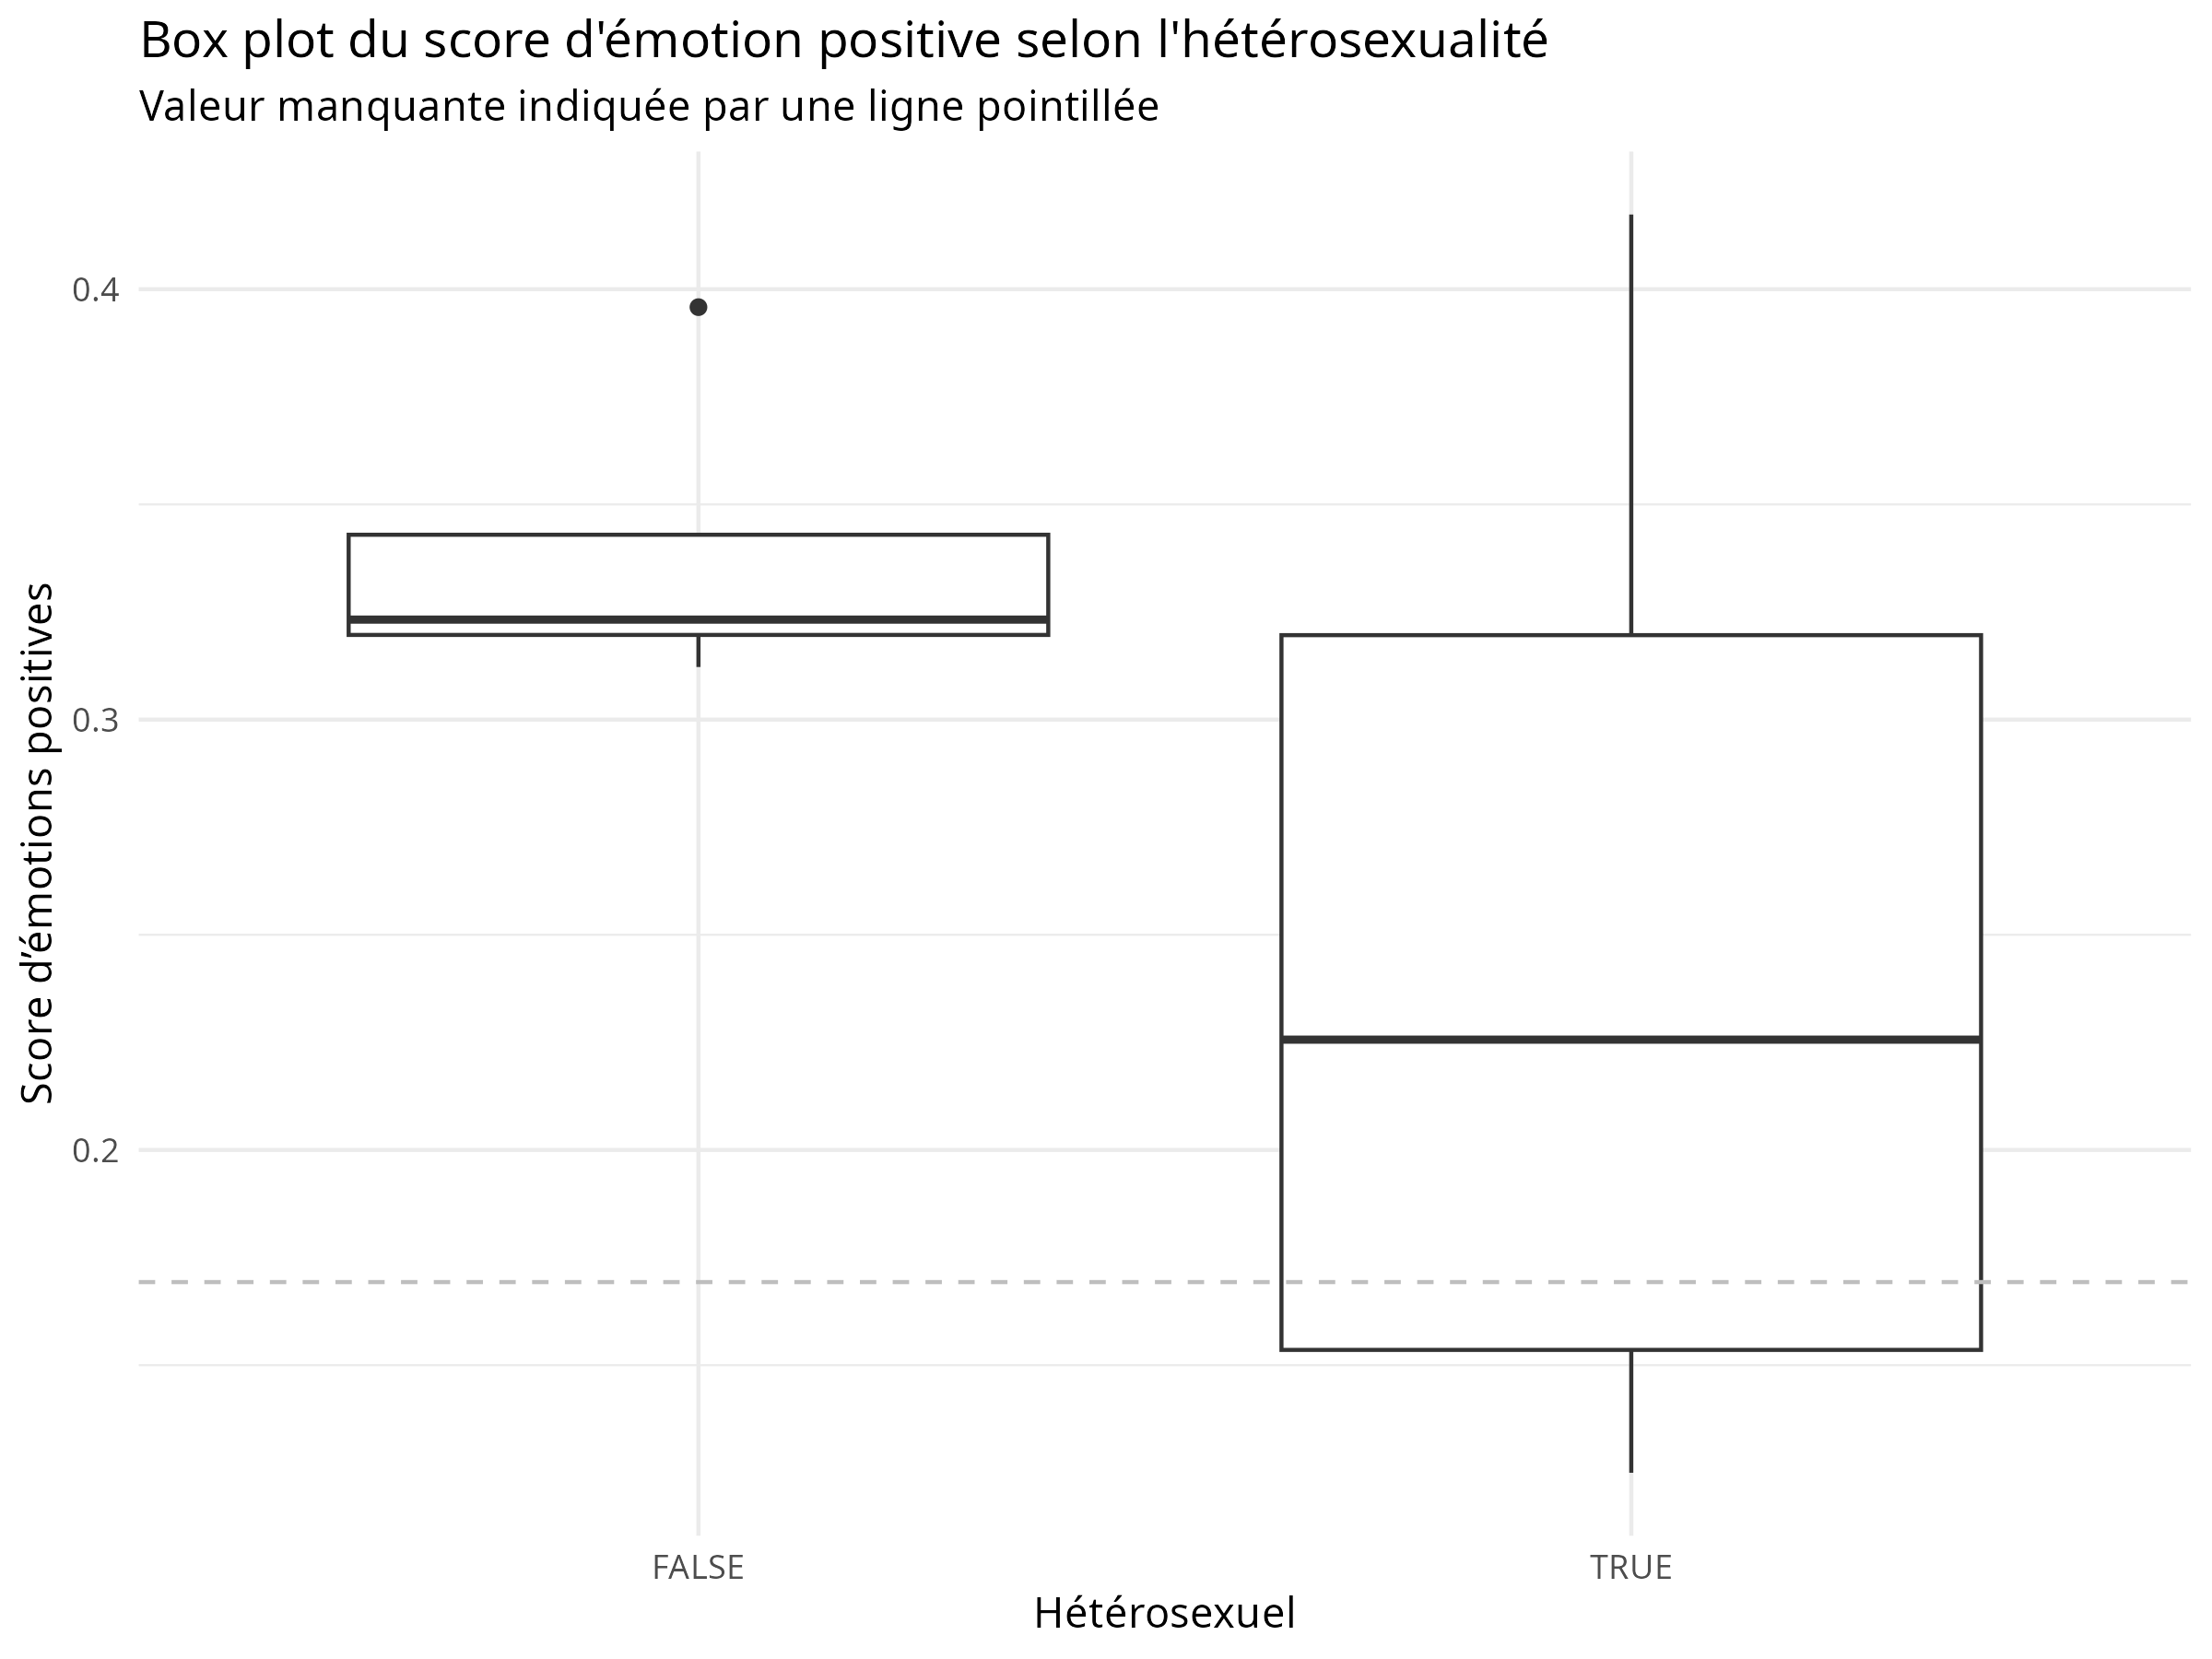
\includegraphics[width=0.8\textwidth]{images/boxplot-positive-heterosexual-missing-values.png}
	\caption{Distribution de \(X\) (score des émotions positives) selon \(Z\) (hétérosexuel ou non). La ligne horizontale indique l’observation pour laquelle \(Z\) est manquant.}
	\label{fig:boxplot-imputation}
\end{figure}

\subsection{Modélisation logistique pour l’imputation}
Pour estimer la probabilité \(\mathbb{P}(Z = 1 \mid X = x)\), on ajuste un modèle de régression logistique binaire sur toutes les observations complètes (celles pour lesquelles la valeur de \(Z\) est connue). Plus précisément, on suppose que :
\[
\mathbb{P}(Z = 1 \mid X = x)
\;=\; \frac{1}{1 + \exp\bigl(-(\beta_0 + \beta_1 x)\bigr)},
\]
où \(\beta_0\) et \(\beta_1\) sont des paramètres inconnus à estimer par la méthode de la vraisemblance maximale.

Une fois ce modèle estimé, la probabilité d’appartenir à la classe \(Z=1\) est calculée pour la poétesse dont la donnée est manquante. Afin de produire une imputation binaire, on convertit cette probabilité en classe \(\hat{z}\in\{0,1\}\) selon la règle de décision suivante :
\[
\hat{z} =
\begin{cases}
	1 & \text{si } \mathbb{P}(Z = 1 \mid X = x) > 0{,}5, \\
	0 & \text{sinon.}
\end{cases}
\]
Dans le présent cas, la probabilité prédite est supérieure à 0,5, ce qui conduit à imputer la valeur \(\hat{z} = 1\) à la poétesse concernée (c’est-à-dire, à la considérer comme hétérosexuelle).

Après ce traitement, la variable \(Z\) ne contient plus aucune valeur manquante, permettant ainsi l’intégration de l’ensemble des poètes (et notamment celui pour lequel l’absence de renseignement posait initialement problème) dans les analyses descriptives et inférentielles. En somme, cette imputation, bien qu’artificielle, facilite l’exploitation globale des données et demeure conforme aux principes de la régression logistique binaire.
